\documentclass[10pt, a4paper]{article}

\usepackage[utf8]{inputenc}
\usepackage{helvet}
\renewcommand{\familydefault}{\sfdefault}
\usepackage[margin=0cm]{geometry}
\usepackage{xcolor}
\usepackage{tikz}
\usepackage{enumitem}
\usepackage{hyperref}
\usepackage{fontawesome5}
\usepackage{graphicx}

% Paleta de colores
\definecolor{headerbg}{HTML}{161E2E}     
\definecolor{sidebarbg}{HTML}{F8FAFC}    
\definecolor{accentblue}{HTML}{0284C7}   
\definecolor{darktext}{HTML}{1E293B}     
\definecolor{lightgray}{HTML}{64748B}    
\definecolor{timelinegray}{HTML}{CBD5E1} 
\definecolor{orcidgreen}{HTML}{A6CE39}   
\definecolor{white}{RGB}{255,255,255}

% Icono ORCID
\newcommand{\orcidicon}{%
    
\begin{tikzpicture}[baseline=-0.5ex]
        \fill[orcidgreen] (0,0) circle (3.8pt);
        \node[text=white, font=\fontsize{4pt}{4pt}\selectfont\bfseries] at (0,0) {iD};
    \end{tikzpicture}%
}

\hypersetup{
    colorlinks=true,
    urlcolor=accentblue,
    linkcolor=accentblue
}

\pagestyle{empty}
\setlength{\parindent}{0pt}

% Comandos visuales
\newcommand{\maintitle}[1]{%
    \vspace{3pt}%
    {\bfseries\fontsize{8.8pt}{10.5pt}\selectfont\color{darktext}\uppercase{#1}}\\[-3pt]%
    {\color{darktext}\rule{\linewidth}{1pt}}\par\vspace{2.5pt}%
}

\newcommand{\sidebadge}[1]{%
    \vspace{4pt}%
    \begin{tikzpicture}
        \node[fill=accentblue, text=white, font=\footnotesize\bfseries, inner sep=2.5pt, rounded corners=2pt] {#1};
    \end{tikzpicture}\par\vspace{2pt}%
}

\newcommand{\timelineentry}[3]{%
    \noindent
    \begin{tikzpicture}[baseline=(entrycontent.north)]
        \node[inner sep=0pt, outer sep=0pt, text width=12.2cm, align=left] (entrycontent) {
            {\fontsize{8.6pt}{10.5pt}\selectfont\textbf{\color{darktext} #1}} \hfill {\scriptsize\color{lightgray} #2}\\[1.5pt]
            #3
        };
        \draw[accentblue, line width=1.3pt] ([xshift=-7pt, yshift=-3.5pt]entrycontent.north west) -- ([xshift=-7pt, yshift=2pt]entrycontent.south west);
        \fill[accentblue] ([xshift=-7pt, yshift=-3.5pt]entrycontent.north west) circle (2.4pt);
    \end{tikzpicture}\par\vspace{2pt}
}

\begin{document}

% BANNER
\begin{tikzpicture}[remember picture, overlay]
    \fill[headerbg] (current page.north west) rectangle ([yshift=-3.4cm]current page.north east);
    \fill[sidebarbg] ([yshift=-3.4cm]current page.north west) rectangle ([xshift=6.7cm]current page.south west);
    \draw[timelinegray, line width=0.6pt] ([xshift=6.7cm, yshift=-3.4cm]current page.north west) -- ([xshift=6.7cm]current page.south west);

    \node[anchor=center, text width=\paperwidth, align=center] at ([yshift=-1.7cm]current page.north) {
        {\fontsize{20pt}{22pt}\selectfont\textbf{\color{white} ARTURO OLIVARES MARTOS}}\\[4pt]
        {\fontsize{9pt}{11pt}\selectfont\textbf{\color{accentblue!40} INGENIERÍA INFORMÁTICA Y MATEMÁTICAS \enspace\textbar\enspace IA \& DATA SCIENCE}}\\[6pt]
        {\fontsize{7.5pt}{9.5pt}\selectfont\color{white!90}
        {\color{accentblue!40}\faMapMarker*} Granada, España \enspace\textbullet\enspace
        {\color{accentblue!40}\faEnvelope} \href{mailto:2004.olivares@gmail.com}{\color{white}2004.olivares@gmail.com} \enspace\textbullet\enspace
        \orcidicon \ \href{https://orcid.org/0009-0000-9415-7268}{\color{white!90}0009-0000-9415-7268} \enspace\textbullet\enspace
        {\color{accentblue!40}\faLinkedin} \href{https://linkedin.com/in/arturo-olivares-martos-4ba54b40a}{\color{white}arturo-olivares-martos} \enspace\textbullet\enspace
        {\color{accentblue!40}\faGithub} \href{https://github.com/arturo-olvrs}{\color{white}arturo-olvrs}
        }
    };
\end{tikzpicture}

\vspace*{3.65cm}

\begin{minipage}[t]{5.8cm}
    \vspace{0pt}\hspace{0.4cm}%
    \begin{minipage}[t]{5.2cm}
        \begin{center}
            \begin{tikzpicture}
                \begin{scope}
                    \clip (0,0) circle (1.3cm);
                    \node at (0,0) {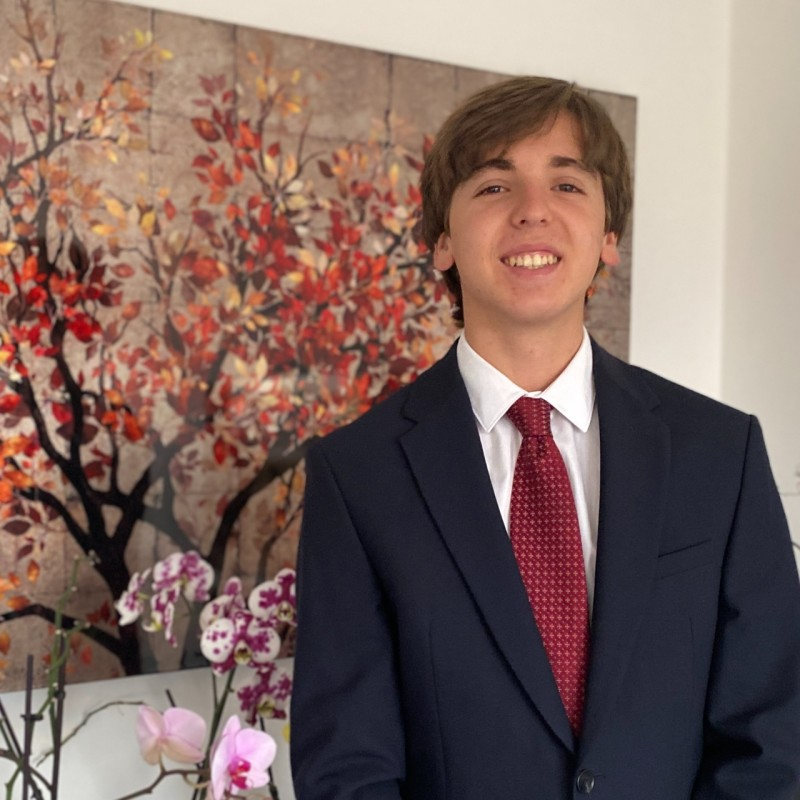
\includegraphics[width=2.6cm, height=2.6cm, keepaspectratio=false]{avatar_temp.jpg}};
                \end{scope}
                \draw[accentblue, line width=2.5pt] (0,0) circle (1.3cm);
            \end{tikzpicture}
        \end{center}
        \vspace{-6pt}

        \sidebadge{SOBRE MÍ}
        {\fontsize{6.8pt}{8.6pt}\selectfont\color{darktext}
        Estudiante de alto rendimiento en UGR con estancia internacional Erasmus en Alemania. Especializado en la convergencia entre modelado matemático riguroso, algoritmia avanzada e ingeniería orientada a IA y MLOps. Trayectoria en investigación, liderazgo comunitario y resolución de problemas complejos.}\par

        \sidebadge{COMPETENCIAS TÉCNICAS}
        {\fontsize{6.8pt}{8.8pt}\selectfont
        \textbf{\color{darktext} Lenguajes \& Frameworks:}\\
        {\color{lightgray} Python, C++, TensorFlow, Scikit-Learn}\\[3pt]
        \textbf{\color{darktext} Modelado \& Matemáticas:}\\
        {\color{lightgray} Optimización, Modelos Estocásticos, Simulación, Algoritmia Avanzada}\\[3pt]
        \textbf{\color{darktext} Data Science \& Herramientas:}\\
        {\color{lightgray} Jupyter, Pandas, NumPy, Análisis de Datos}\\[3pt]
        \textbf{\color{darktext} Infraestructura \& DevOps:}\\
        {\color{lightgray} Git, GitHub, CI/CD, Docker, Google Cloud (GCP / MLOps)}
        }\par

        \sidebadge{TÍTULOS DE IDIOMAS}
        {\scriptsize\textbf{\color{darktext} Inglés:}} {\scriptsize\color{lightgray} C2 Proficiency (Cambridge)}\\[1.5pt]
        {\scriptsize\textbf{\color{darktext} Alemán:}} {\scriptsize\color{lightgray} C1 (Goethe-Zertifikat)}\\[1.5pt]
        {\scriptsize\textbf{\color{darktext} Francés:}} {\scriptsize\color{lightgray} B2 (DELF Internacional)}\\[1.5pt]
        {\scriptsize\textbf{\color{darktext} Español:}} {\scriptsize\color{lightgray} Nativo}

        \sidebadge{INMERSIÓN EN EL EXTRANJERO}
        {\fontsize{6.6pt}{8.2pt}\selectfont
        \textbf{\color{darktext} Inmersión en Berlín (Alemania)}\\
        {\color{lightgray} GLS German Language School · Nivel B2.2 (2024)}\\[2.5pt]
        \textbf{\color{darktext} Inmersión en Exmouth (UK)}\\
        {\color{lightgray} Hello! Exmouth · Nivel B2+ (2019)}\\[2.5pt]
        \textbf{\color{darktext} Inmersión en Múnich (Alemania)}\\
        {\color{lightgray} Landheim Ammersee · International Summer School · Nivel B1 (2019)}\\[2.5pt]
        \textbf{\color{darktext} Young Professionals en Oxford (UK)}\\
        {\color{lightgray} d'Overbroeck's · Engineering Course (2018)}
        }\par

        \sidebadge{CERTIFICACIONES}
        {\fontsize{6.6pt}{8.2pt}\selectfont
        \textbf{\color{darktext} MLOps for Generative AI}\\
        {\color{lightgray} Google Cloud Skills Boost · 2026}\\[2pt]
        \textbf{\color{darktext} Lógica y Teoría de Conjuntos}\\
        {\color{lightgray} Microcredencial UGR · 2025}\\[2pt]
        \textbf{\color{darktext} Monitor de Actividades en el Tiempo Libre Infantil y Juvenil}\\
        {\color{lightgray} Junta de Andalucía · 2022}
        }\par
    \end{minipage}
\end{minipage}%
\hfill
\begin{minipage}[t]{13.1cm}
    \vspace{0pt}

    \maintitle{EDUCACIÓN Y RENDIMIENTO ACADÉMICO}

    \timelineentry{Doble Grado en Ing. Informática y Matemáticas}{2022 -- 2027}{%
        {\footnotesize\textbf{\color{accentblue} Universidad de Granada (UGR)}} \hfill {\scriptsize\color{lightgray} Granada, España}\\[1.5pt]
        \begin{itemize}[leftmargin=*, nosep, topsep=1pt, itemsep=1.5pt]
            \item \textbf{Nota media de expediente: 9,2 / 10}.
            \item Especialización en IA, Ciencia de Datos y Optimización Matemática.
        \end{itemize}
    }

    \timelineentry{Programa Erasmus+ \textbar\ Computer Science \& Data Science}{2025 -- 2026}{%
        {\footnotesize\textbf{\color{accentblue} University of Duisburg-Essen}} \hfill {\scriptsize\color{lightgray} Duisburg, Alemania}\\[1.5pt]
        \begin{itemize}[leftmargin=*, nosep, topsep=1pt, itemsep=1.5pt]
            \item Estancia internacional; materias de posgrado en modelado e IA.
        \end{itemize}
    }

    \timelineentry{Bachillerato de Ciencias y Tecnología}{2020 -- 2022}{%
        {\footnotesize\textbf{\color{accentblue} HH. Maristas Granada}} \hfill {\scriptsize\color{lightgray} Granada, España}\\[1.5pt]
        \begin{itemize}[leftmargin=*, nosep, topsep=1pt, itemsep=1.5pt]
            \item \textbf{2.ª mejor nota de Selectividad (PEvAU)} en la provincia de Granada (\textbf{13,975 / 14,000}).
        \end{itemize}
    }

    \timelineentry{Bachillerato Dual Americano (High School Diploma)}{2019 -- 2022}{%
        {\footnotesize\textbf{\color{accentblue} Academica International Studies}} \hfill {\scriptsize\color{lightgray} EE. UU. / Online}
    }

    \vspace{3pt}

    \maintitle{LIDERAZGO Y COMUNIDAD DIGITAL}

    \timelineentry{Fundador y Coordinador Principal}{Sept. 2022 -- Actualidad}{%
        {\footnotesize\textbf{\color{accentblue} Los Del DGIIM (Comunidad UGR)}} \hfill {\scriptsize\color{lightgray} Granada, España}\\[1.5pt]
        \begin{itemize}[leftmargin=*, nosep, topsep=1pt, itemsep=1.5pt]
            \item Fundación de la red comunitaria del Doble Grado; moderación de canales oficiales con cientos de alumnos.
            \item Administración de repositorios GitHub con código, apuntes y arquitecturas de uso masivo.
        \end{itemize}
    }

    \maintitle{INVESTIGACIÓN, CONGRESOS Y DIVULGACIÓN}

    \begin{itemize}[leftmargin=*, nosep, topsep=1pt, itemsep=2pt]
        \item \href{https://doi.org/10.5334/jors.771}{\textbf{\color{darktext}\footnotesize Making Soundscape Assessment Accessible: The SoundGraphy Tool \faExternalLink*}} \hfill {\scriptsize\color{lightgray} Sept. 2026}\\
        {\scriptsize\textit{Journal of Open Research Software (JORS) -- Ubiquity Press (Vol. 14: 63)}}\\
        {\scriptsize Primer autor y desarrollador de software para análisis de paisaje sonoro (ISO 12913 y SSM).}
        \item \href{https://dl.gi.de/items/4b863f76-35d4-4ec3-a18b-427b56539919}{\textbf{\color{darktext}\footnotesize Monitoring and Understanding Notebook-Based Learning with Jupyter \faExternalLink*}} \hfill {\scriptsize\color{lightgray} Duisburg · Sept. 2026}\\
        {\scriptsize\textit{Mensch und Computer (MuC 2026) -- Gesellschaft für Informatik e.V. (GI)}}\\
        {\scriptsize Coautor de investigación en analítica del aprendizaje y dashboards.}
        \item \textbf{\color{darktext}\footnotesize Delegado Universitario en Congreso AIvolution} \hfill {\scriptsize\color{lightgray} Bruselas · 2023}\\
        {\scriptsize\textit{Parlamento Europeo (Renew Europe)}: Seleccionado para debatir con expertos internacionales sobre el impacto socioeconómico de la IA, derechos digitales, ciberseguridad y regulación tecnológica.}
        \item \href{https://revistasuma.es/wp-content/uploads/suma/Suma104/S104w_039-052.pdf}{\textbf{\color{darktext}\footnotesize Modelado matemático, vacunación y Python \faExternalLink*}} \hfill {\scriptsize\color{lightgray} Granada · Ago. 2022}\\
        {\scriptsize\textit{Revista científica SUMA+ (N.º 104, pp. 39-52)}: Optimización logística y distribución frente al COVID-19.}
        \item \textbf{\color{darktext}\footnotesize Ponente Formativo en Modelado Computacional} \hfill {\scriptsize\color{lightgray} CEFIRE Valencia · Febr. 2021}\\
        {\scriptsize Sesiones técnicas para docentes sobre aplicaciones reales de modelado matemático y simulación.}
    \end{itemize}

    \maintitle{PREMIOS Y MÉRITOS DESTACADOS}

    \begin{itemize}[leftmargin=*, nosep, topsep=1pt, itemsep=1.5pt]
        \item \textbf{\color{darktext}\footnotesize Bicampeón Nacional y Doble Mención de Honor Mundial -- IMMC} \hfill {\scriptsize\color{lightgray} 2020, 2021}\\
        {\scriptsize 1.er puesto de España (2 años consecutivos) y Mención de Honor Global en el \textit{IMMC} por optimización multivariable.}
        \item \textbf{\color{darktext}\footnotesize 1.er Premio Nacional de Química (\#STEM\_for\_Teens)} \hfill {\scriptsize\color{lightgray} Abr. 2019}\\
        {\scriptsize Reconocimiento nacional otorgado por Google, Real Academia de Ciencias y Junior Achievement.}
        \item \textbf{\color{darktext}\footnotesize Accésit XXXIV Olimpiada Matemática THALES} \hfill {\scriptsize\color{lightgray} Abr. 2018}
    \end{itemize}

    \maintitle{COMPROMISO SOCIAL Y VOLUNTARIADO}

    \begin{itemize}[leftmargin=*, nosep, topsep=1pt, itemsep=1.5pt]
        \item \textbf{\footnotesize Student Volunteer:} Congreso MuC 2026 (Sociedad Alemana de Informática). \hfill {\scriptsize\color{lightgray} Ago. 2026}
        \item \textbf{\footnotesize Monitor de Juventud y Tiempo Libre:} Maristas Provincia Mediterránea. \hfill {\scriptsize\color{lightgray} 2021 -- Actualidad}
        \item \textbf{\footnotesize Acción Social:} Comedor Social Hijas de la Caridad y Asoc. Autismo Córdoba.
    \end{itemize}

\end{minipage}
\hspace{0.4cm}

\end{document}